\documentclass[12pt,a4papaer]{article}
\usepackage[legalpaper, margin=1.2in]{geometry}

\usepackage[utf8]{inputenc}
\usepackage[hidelinks]{hyperref}
\usepackage{bera}% optional: just to have a nice mono-spaced font
\usepackage{listings}
\usepackage{xcolor}
\usepackage{graphicx}

\graphicspath{ {./img/} }

\setlength{\parindent}{5ex}

\colorlet{punct}{red!60!black}
\definecolor{background}{HTML}{EEEEEE}
\definecolor{delim}{RGB}{20,105,176}

\lstdefinelanguage{json}{
    basicstyle=\normalfont\ttfamily,
    basicstyle=\scriptsize,
    showstringspaces=false,
    breaklines=true,
    frame=lines,
    backgroundcolor=\color{background},
    literate=
     *{:}{{{\color{punct}{:}}}}{1}
      {,}{{{\color{punct}{,}}}}{1}
      {;}{{{\color{punct}{,}}}}{1}
      {\{}{{{\color{delim}{\{}}}}{1}
      {\}}{{{\color{delim}{\}}}}}{1}
      {[}{{{\color{delim}{[}}}}{1}
      {]}{{{\color{delim}{]}}}}{1}
      {(}{{{\color{delim}{(}}}}{1}
      {)}{{{\color{delim}{)}}}}{1},
}

\title{SAP Hana és Python integráció}
\date{2020. 04. 11.}
\author{Cseresnyés Bendegúz (ENVDUV)}
\begin{document}



    \maketitle
    \tableofcontents

    \newpage
    \section{A választott dataset és az adatok előfeldolgozása}
    \subsection{Dataset}
    A COVID-19 nevű vírus 2019 decemberében jelent meg Kínában és néhány hónapon belül az egész világon elterjedt.
    Egy ilyen világméretű katasztrófának tekinthető betegség rendkívül sok embert foglalkoztat, precízen követik és dokumentálják a pontos fertőzöttségi adatokat.
    Ezen adatok egy kis szeletével szeretnék ebben a tanulmányban foglalkozni, vizsgálni a terjedését adott területeken és a vilgágon.
    Az adatokat a következő Dataset biztosítja: \hyperref[dataset_link]{URL} .

    \subsection{Adatok szerkezete}
    A CSV fájlokban a táblázatok a következő oszlopokat tartalmazzák: Tartomány, Ország, Jelentés dátuma, Igazolt fertőzöttek száma, Feltételezetten fertőzöttek száma, Gyógyultak száma, Elhunytak száma.
    Ezek a fájlok 8 napi adatról állnak rendelkezésemre, az adatok 2020. 01. 21. és 2020. 02. 06. közöttiek.
    Az adatok legnagyobb problémája a felhasználás szempontjából, hogy az egyes területek jelentései közt akár napok is elteltek anélkül, hogy rögzítve lett volna az aktuális érték a táblázatban, 
    nem adott időpontokhoz vannak rögzítve a mérési eredmények, eltérő dátum és idő formátumot használnak a fájl több pontján.
    \subsection{Előfeldolgozás}
    Az imént említett dástum formázási probléma miatt az adatokat nem is tudtam importálni a rendszerbe, ezért egységesíteni kellett a dátum formátumokat.
    Legegyszerűbb megoldást ebben az esetben a fájlok kis száma miatt egy-egy egyszerűbb reguláris kifejezés alapján történő csere jelentette számomra.
    Átfutottam az adatokat, hogy milyen formázások fordulnak elő, és az egyes típusokra megadtam az arra illeszkedő kifejezést, majd a paramétereket újra összeillesztettem megfelelő formában.
    \subsubsection{Példa a formázásra: }
        \begin{verbatim}
        Eredeti sor: Hubei,Mainland China,2/5/20 16:43,16678,,538,479
        Kimeneti sor: Hubei,Mainland China,2020-2-5 16:43,16678,,538,479
        Kereső kifejezés: ,(\d{1,2})/(\d{1,2})/20 [^,]*
        Helyettesítés: 2020-$1-$2 $3
        \end{verbatim}
    \subsection{Adatok tárolása és importálása}

    Az adatokat a CSV fájllal megegyező tábla struktúrában tárolom, kiegészítve egy source\_id nevű mezővel ami az automatikus importálás miatt szükséges, 
    e nélkül az importálás nem tud végigmenni, mivel a fájlok között vannak egyező adattartalmú sorok, amik hibát generálnának az importálás során.
    Ennek a mezőnek az értékét az importáls során konstans értékre beállítom, minden fájlhoz különböző egész számot rendelve.
    A többi mező értéke a neki megfelelő oszlop tartalma alapján kerül beállításra.
    Az importálás kódja megtalálható az upload\_tabledata.htbtabledata fileban.

    \par
    Az adatokat a Covid\_raw nevű tábja tárolja. Az ország és tartomány neveket szövegesen, a frissítés dátumát dátum és idő formátumban, a fertőzöttségi adatokat számként.

    \subsubsection{Covid\_raw.hdbtable}
    \begin{lstlisting}[language=json]
        column table "envduv_COVID_visual.db.data::Covid_raw" (
            "province"    VARCHAR(256)	CS_STRING,
            "region"      VARCHAR(256)	CS_STRING,
            "last_update" TIMESTAMP CS_LONGDATE,
            "confirmed"   DOUBLE CS_DOUBLE,
            "suspected"   DOUBLE CS_DOUBLE,
            "recovered"   DOUBLE CS_DOUBLE,
            "death"       DOUBLE CS_DOUBLE,
            "source_id"   INTEGER CS_INT
        );
    \end{lstlisting}
    \subsubsection{Részlet az upload\_tabledata.hdbtabledata fileból:}
    \begin{lstlisting}[language=json]
        {
            "column_mappings" : { 
                "province": "Province/State",
                "region": "Country/Region",
                "last_update": "Last Update",
                "confirmed": "Confirmed",
                "suspected": "Suspected",
                "recovered": "Recovered",
                "death": "Death",
                "source_id": { "type": "constant", "value": "2" }
            },
            "import_settings" : { 
                "import_columns" : [ 
                    "province",
                    "region",
                    "last_update",
                    "confirmed",
                    "suspected",
                    "recovered",
                    "death",
                    "source_id"
                ]
            },
            "source_data" : {
                "data_type" : "CSV", 
                "has_header" : true, 
                "dialect" : "HANA", 
                "type_config" : { "delimiter" : ";", "do_quote": false },
                "file_name" : "envduv_COVID_visual.db.data_source::2019_nCoV_20200121_20200127.csv"
            },
            "target_table" : "envduv_COVID_visual.db.data::Covid_raw"  
        },
    \end{lstlisting}

    \subsection{Idősor adatok előállítása}
    Az adatok felhasználhatósága érdeekében egy folyamatos idősor előállítására volt szükség, 
    ahol egységes időközönként minden területhez hozzá rendeli a legutolsó fertőzöttségi adatot a minták közül.
    A nyers adatok alapján létrehoztam egy nézetet, ami az összes elérhető időpont alapján napi 4 időpontot 
    határoz meg a mérések kiértékelésére, ha az adott szegmenshez tartozik mért adat.
    A nyers adatok alapján egy másik nézet listázza az összes elérhető tartomány-ország párt, ezeken a helyeken 
    fogjuk kiértékelni a legutolsó mérés eredményét az összes előbb meghatázozott időpillanatban.
    Kezdetben csak az idő alapján rendeztem az adott szegmensekhez a mérési eredményeket, 
    de ez eltéréshez vezetett a különböző kiértékelések között 
    (például csoportosítással és csoportosítás nélkül keresett maximum esetén jött elő olyan hiba, hogy a legmagasabb tartománynak nem volt azonos az értéke a 2 lekérdezés során).
    Mivel nem minden méréshez állt rendelkezésre a pontos mérési idő, hanem csak a dátum, ezért kiértékeléstől függően változott, hogy az adatbázis melyik eredményt nézte az ilyen csoportoknál.
    Emiatt került be, hogy az egyes időpontokhoz nem csak mérési idő szerint rendezem a tételeket, hanem igazolt esetek száma szerint is, 
    így biztosítva, hogy mindig csak 1 legközelebbi mérési eredmény alapján kerüljön meghatározásra a keresett időpont.

    \subsubsection{CovidTimeSeries.hdbview}
    \begin{lstlisting}[language=json]
VIEW "envduv_COVID_visual.db.data::CovidTimeSeries" AS
SELECT DISTINCT
	s."region", s."province", s."timestamp", 
	first_value( d."last_update") over (partition by s."region", s."province", s."timestamp" order by d."last_update" desc) as "last_update",
    first_value( d."confirmed") over (partition by s."region", s."province", s."timestamp" order by d."last_update" desc) as "confirmed",
    ...
FROM "envduv_COVID_visual.db.data::Samples" as s left outer join "envduv_COVID_visual.db.data::Covid_raw" d
on 
	(s."region" = d."region" or (s."region" is null and d."region" is null)) and 
	(s."province" = d."province" or (s."province" is null and d."province" is null)) and 
	s."timestamp" >= d."last_update"
order by s."province"
    \end{lstlisting}

    \subsubsection{Vírus terjedése táblázatosan a világ összes esetét figyelembe véve}
    \begin{center}
        \begin{tabular}{|c c c c c|}
            \hline
            Időpont& Igazolt& Gyanús& Gyúgyult& Elhunyt \\
            \hline
            2020-01-21 00:00:00.000000000&333&286& & \\
            2020-01-22 12:00:00.000000000&558&254& & \\
            2020-01-23 12:00:00.000000000&656&261&30&18 \\
            2020-01-24 00:00:00.000000000&884&244&34&26 \\
            2020-01-24 12:00:00.000000000&943&288&36&26 \\
            2020-01-25 00:00:00.000000000&1360&197&38&41 \\
            2020-01-25 12:00:00.000000000&1692&530&39&43 \\
            2020-01-25 18:00:00.000000000&1692&530&39&43 \\
            2020-01-26 06:00:00.000000000&2025&530&49&55 \\
            2020-01-26 18:00:00.000000000&2123&507&52&56 \\
            2020-01-27 06:00:00.000000000&2801&124&54&80 \\
            ... \\
            \hline
        \end{tabular}
    \end{center}
    \subsubsection{Vírus terjedése vonal grafikonnal}
    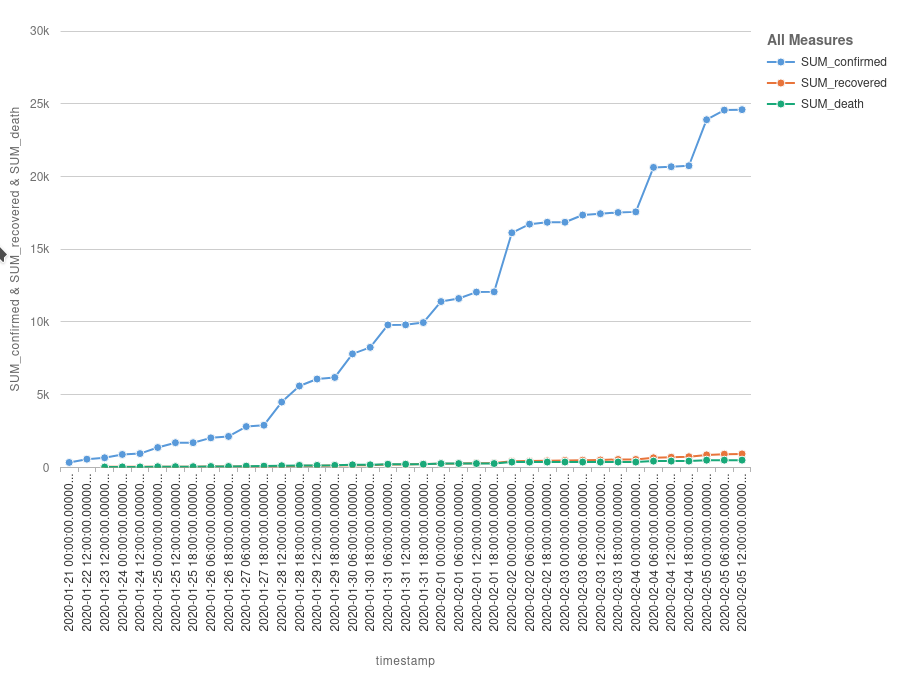
\includegraphics[width=\textwidth]{sum_ww}
    \subsection{Adatok hozzáférhetővé tétele}
    \subsection{Elemzési eredmények tárolása}
    \newpage
    \section{Python}
    \subsection{Adatbázis kapcsolat kiépítése}
    \subsection{Elemzés pythonban}
    \subsection{Flask: api hívás elemző algoritmus futtatására}
    \subsection{Python scriptek futtatása HANA környezetben}

    \newpage
    \section{Analitikai eredmények vizualizálása}
    \subsection{Adatok elérése ODATA interfészen keresztül}
    \subsection{Adatok vizualizálása SAP rendszereken}

    \newpage
    \section{Felhasznált források}
    \begin{itemize}
        \item https://hu.wikipedia.org/wiki/LaTeX
        \item \label{dataset_link} \url{ https://www.kaggle.com/therealcyberlord/coronavirus-covid-19-visualization-prediction/data}
    \end{itemize}
\end{document}